\documentclass[tikz,border=10pt]{standalone}
\usetikzlibrary{calc}

\begin{document}
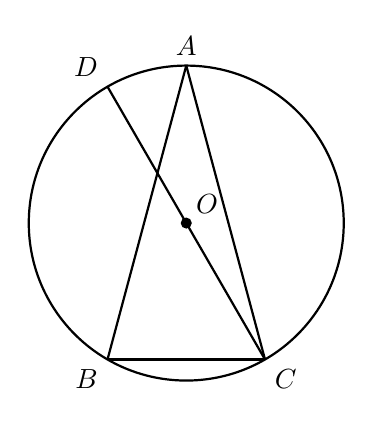
\begin{tikzpicture}
    % --- 参数定义 ---
    \def\R{2} % 设置圆的半径

    % --- 绘制圆 ---
    \draw[thick] (0,0) circle (\R);
    \fill (0,0) circle (2pt) node[above right] {$O$};

    % --- 定义坐标 ---
    % 使用极坐标定位圆周上的点
    \coordinate (A) at (90:\R);
    \coordinate (B) at (240:\R);
    \coordinate (C) at (300:\R);
    \coordinate (D) at (120:\R); % 保证 D, O, C 三点共线

    % --- 绘制线段 ---
    \draw[thick] (B) -- (C);      % 弦 BC
    \draw[thick] (A) -- (B);      % 边 AB
    \draw[thick] (A) -- (C);      % 边 AC
    \draw[thick] (D) -- (C);      % 直径 DC (经过圆心)

    % --- 标注点 ---
    \node[above] at (A) {$A$};
    \node[below left] at (B) {$B$};
    \node[below right] at (C) {$C$};
    \node[above left] at (D) {$D$};

\end{tikzpicture}
\end{document}